% Created by tikzDevice version 0.12 on 2019-04-26 11:42:01
% !TEX encoding = UTF-8 Unicode
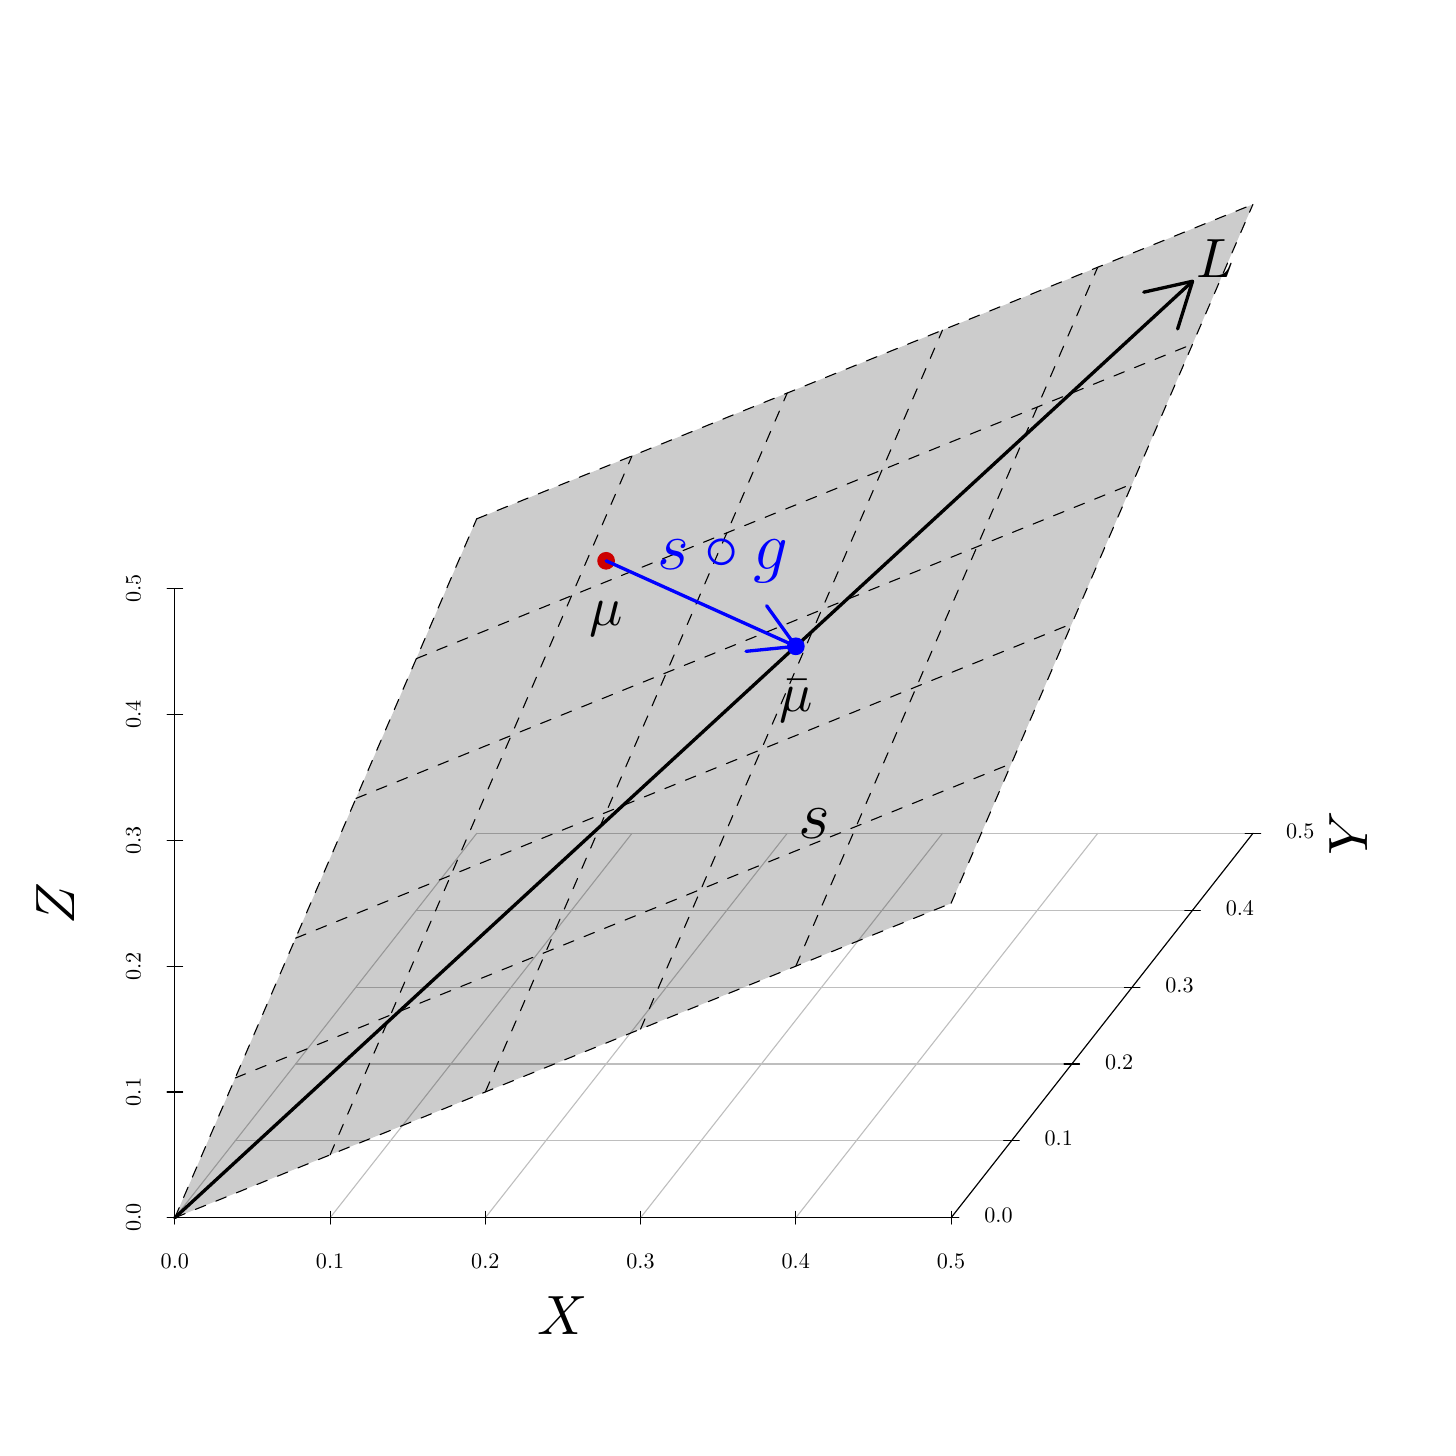
\begin{tikzpicture}[x=1pt,y=1pt]
\definecolor{fillColor}{RGB}{255,255,255}
\path[use as bounding box,fill=fillColor,fill opacity=0.00] (0,0) rectangle (505.89,505.89);
\begin{scope}
\path[clip] ( 37.20, 61.20) rectangle (468.69,456.69);
\definecolor{drawColor}{RGB}{190,190,190}

\path[draw=drawColor,line width= 0.4pt,line join=round,line cap=round] ( 53.18, 75.85) -- (162.26,214.75);

\path[draw=drawColor,line width= 0.4pt,line join=round,line cap=round] (109.28, 75.85) -- (218.36,214.75);

\path[draw=drawColor,line width= 0.4pt,line join=round,line cap=round] (165.38, 75.85) -- (274.45,214.75);

\path[draw=drawColor,line width= 0.4pt,line join=round,line cap=round] (221.47, 75.85) -- (330.55,214.75);

\path[draw=drawColor,line width= 0.4pt,line join=round,line cap=round] (277.57, 75.85) -- (386.65,214.75);

\path[draw=drawColor,line width= 0.4pt,line join=round,line cap=round] (333.67, 75.85) -- (442.74,214.75);

\path[draw=drawColor,line width= 0.4pt,line join=round,line cap=round] ( 53.18, 75.85) -- (333.67, 75.85);

\path[draw=drawColor,line width= 0.4pt,line join=round,line cap=round] ( 75.00,103.63) -- (355.48,103.63);

\path[draw=drawColor,line width= 0.4pt,line join=round,line cap=round] ( 96.81,131.41) -- (377.30,131.41);

\path[draw=drawColor,line width= 0.4pt,line join=round,line cap=round] (118.63,159.19) -- (399.11,159.19);

\path[draw=drawColor,line width= 0.4pt,line join=round,line cap=round] (140.44,186.97) -- (420.93,186.97);

\path[draw=drawColor,line width= 0.4pt,line join=round,line cap=round] (162.26,214.75) -- (442.74,214.75);
\definecolor{drawColor}{RGB}{0,0,0}

\path[draw=drawColor,line width= 0.4pt,line join=round,line cap=round] (330.86, 75.85) -- (336.47, 75.85);

\path[draw=drawColor,line width= 0.4pt,line join=round,line cap=round] (352.68,103.63) -- (358.29,103.63);

\path[draw=drawColor,line width= 0.4pt,line join=round,line cap=round] (374.49,131.41) -- (380.10,131.41);

\path[draw=drawColor,line width= 0.4pt,line join=round,line cap=round] (396.31,159.19) -- (401.92,159.19);

\path[draw=drawColor,line width= 0.4pt,line join=round,line cap=round] (418.12,186.97) -- (423.73,186.97);

\path[draw=drawColor,line width= 0.4pt,line join=round,line cap=round] (439.94,214.75) -- (445.55,214.75);

\path[draw=drawColor,line width= 0.4pt,line join=round,line cap=round] ( 53.18, 73.57) -- ( 53.18, 78.12);

\path[draw=drawColor,line width= 0.4pt,line join=round,line cap=round] (109.28, 73.57) -- (109.28, 78.12);

\path[draw=drawColor,line width= 0.4pt,line join=round,line cap=round] (165.38, 73.57) -- (165.38, 78.12);

\path[draw=drawColor,line width= 0.4pt,line join=round,line cap=round] (221.47, 73.57) -- (221.47, 78.12);

\path[draw=drawColor,line width= 0.4pt,line join=round,line cap=round] (277.57, 73.57) -- (277.57, 78.12);

\path[draw=drawColor,line width= 0.4pt,line join=round,line cap=round] (333.67, 73.57) -- (333.67, 78.12);

\path[draw=drawColor,line width= 0.4pt,line join=round,line cap=round] ( 50.38, 75.85) -- ( 55.99, 75.85);

\path[draw=drawColor,line width= 0.4pt,line join=round,line cap=round] ( 50.38,121.31) -- ( 55.99,121.31);

\path[draw=drawColor,line width= 0.4pt,line join=round,line cap=round] ( 50.38,166.77) -- ( 55.99,166.77);

\path[draw=drawColor,line width= 0.4pt,line join=round,line cap=round] ( 50.38,212.22) -- ( 55.99,212.22);

\path[draw=drawColor,line width= 0.4pt,line join=round,line cap=round] ( 50.38,257.68) -- ( 55.99,257.68);

\path[draw=drawColor,line width= 0.4pt,line join=round,line cap=round] ( 50.38,303.14) -- ( 55.99,303.14);
\end{scope}
\begin{scope}
\path[clip] (  0.00,  0.00) rectangle (505.89,505.89);
\definecolor{drawColor}{RGB}{0,0,0}

\node[text=drawColor,anchor=base,inner sep=0pt, outer sep=0pt, scale=  0.80] at ( 53.18, 57.60) {0.0};

\node[text=drawColor,anchor=base,inner sep=0pt, outer sep=0pt, scale=  0.80] at (109.28, 57.60) {0.1};

\node[text=drawColor,anchor=base,inner sep=0pt, outer sep=0pt, scale=  0.80] at (165.38, 57.60) {0.2};

\node[text=drawColor,anchor=base,inner sep=0pt, outer sep=0pt, scale=  0.80] at (221.47, 57.60) {0.3};

\node[text=drawColor,anchor=base,inner sep=0pt, outer sep=0pt, scale=  0.80] at (277.57, 57.60) {0.4};

\node[text=drawColor,anchor=base,inner sep=0pt, outer sep=0pt, scale=  0.80] at (333.67, 57.60) {0.5};

\node[text=drawColor,rotate= 90.00,anchor=base,inner sep=0pt, outer sep=0pt, scale=  0.80] at ( 40.80, 75.85) {0.0};

\node[text=drawColor,rotate= 90.00,anchor=base,inner sep=0pt, outer sep=0pt, scale=  0.80] at ( 40.80,121.31) {0.1};

\node[text=drawColor,rotate= 90.00,anchor=base,inner sep=0pt, outer sep=0pt, scale=  0.80] at ( 40.80,166.77) {0.2};

\node[text=drawColor,rotate= 90.00,anchor=base,inner sep=0pt, outer sep=0pt, scale=  0.80] at ( 40.80,212.22) {0.3};

\node[text=drawColor,rotate= 90.00,anchor=base,inner sep=0pt, outer sep=0pt, scale=  0.80] at ( 40.80,257.68) {0.4};

\node[text=drawColor,rotate= 90.00,anchor=base,inner sep=0pt, outer sep=0pt, scale=  0.80] at ( 40.80,303.14) {0.5};
\end{scope}
\begin{scope}
\path[clip] ( 37.20, 61.20) rectangle (468.69,456.69);
\definecolor{drawColor}{RGB}{0,0,0}

\node[text=drawColor,anchor=base west,inner sep=0pt, outer sep=0pt, scale=  0.80] at (345.67, 74.01) {0.0};

\node[text=drawColor,anchor=base west,inner sep=0pt, outer sep=0pt, scale=  0.80] at (367.48,101.79) {0.1};

\node[text=drawColor,anchor=base west,inner sep=0pt, outer sep=0pt, scale=  0.80] at (389.30,129.57) {0.2};

\node[text=drawColor,anchor=base west,inner sep=0pt, outer sep=0pt, scale=  0.80] at (411.11,157.35) {0.3};

\node[text=drawColor,anchor=base west,inner sep=0pt, outer sep=0pt, scale=  0.80] at (432.93,185.13) {0.4};

\node[text=drawColor,anchor=base west,inner sep=0pt, outer sep=0pt, scale=  0.80] at (454.74,212.91) {0.5};

\path[draw=drawColor,line width= 0.4pt,line join=round,line cap=round] ( 53.18, 75.85) --
	(333.67, 75.85);
\end{scope}
\begin{scope}
\path[clip] (  0.00,  0.00) rectangle (505.89,505.89);
\definecolor{drawColor}{RGB}{0,0,0}

\node[text=drawColor,anchor=base,inner sep=0pt, outer sep=0pt, scale=  2.00] at (193.42, 33.60) {$X$};
\end{scope}
\begin{scope}
\path[clip] ( 37.20, 61.20) rectangle (468.69,456.69);
\definecolor{drawColor}{RGB}{0,0,0}

\path[draw=drawColor,line width= 0.4pt,line join=round,line cap=round] (333.67, 75.85) --
	(442.74,214.75);
\end{scope}
\begin{scope}
\path[clip] (  0.00,  0.00) rectangle (505.89,505.89);
\definecolor{drawColor}{RGB}{0,0,0}

\node[text=drawColor,rotate= 90.00,anchor=base,inner sep=0pt, outer sep=0pt, scale=  2.00] at (484.29,214.75) {$Y$};
\end{scope}
\begin{scope}
\path[clip] ( 37.20, 61.20) rectangle (468.69,456.69);
\definecolor{drawColor}{RGB}{0,0,0}

\path[draw=drawColor,line width= 0.4pt,line join=round,line cap=round] ( 53.18, 75.85) --
	( 53.18,303.14);
\end{scope}
\begin{scope}
\path[clip] (  0.00,  0.00) rectangle (505.89,505.89);
\definecolor{drawColor}{RGB}{0,0,0}

\node[text=drawColor,rotate= 90.00,anchor=base,inner sep=0pt, outer sep=0pt, scale=  2.00] at ( 16.80,189.49) {$Z$};
\end{scope}
\begin{scope}
\path[clip] ( 37.20, 61.20) rectangle (468.69,456.69);
\definecolor{drawColor}{RGB}{255,0,0}
\definecolor{fillColor}{RGB}{255,0,0}

\path[draw=drawColor,line width= 0.4pt,line join=round,line cap=round,fill=fillColor] (209.01,313.24) circle (  3.00);
\definecolor{fillColor}{RGB}{0,0,0}

\path[fill=fillColor,fill opacity=0.20] ( 53.18, 75.85) --
	(162.26,328.40) --
	(442.74,442.04) --
	(333.67,189.49) --
	cycle;
\definecolor{drawColor}{RGB}{0,0,0}

\path[draw=drawColor,line width= 0.4pt,dash pattern=on 4pt off 4pt ,line join=round,line cap=round] ( 53.18, 75.85) -- (162.26,328.40);

\path[draw=drawColor,line width= 0.4pt,dash pattern=on 4pt off 4pt ,line join=round,line cap=round] (109.28, 98.58) -- (218.36,351.12);

\path[draw=drawColor,line width= 0.4pt,dash pattern=on 4pt off 4pt ,line join=round,line cap=round] (165.38,121.31) -- (274.45,373.85);

\path[draw=drawColor,line width= 0.4pt,dash pattern=on 4pt off 4pt ,line join=round,line cap=round] (221.47,144.04) -- (330.55,396.58);

\path[draw=drawColor,line width= 0.4pt,dash pattern=on 4pt off 4pt ,line join=round,line cap=round] (277.57,166.77) -- (386.65,419.31);

\path[draw=drawColor,line width= 0.4pt,dash pattern=on 4pt off 4pt ,line join=round,line cap=round] (333.67,189.49) -- (442.74,442.04);

\path[draw=drawColor,line width= 0.4pt,dash pattern=on 4pt off 4pt ,line join=round,line cap=round] ( 53.18, 75.85) -- (333.67,189.49);

\path[draw=drawColor,line width= 0.4pt,dash pattern=on 4pt off 4pt ,line join=round,line cap=round] ( 75.00,126.36) -- (355.48,240.00);

\path[draw=drawColor,line width= 0.4pt,dash pattern=on 4pt off 4pt ,line join=round,line cap=round] ( 96.81,176.87) -- (377.30,290.51);

\path[draw=drawColor,line width= 0.4pt,dash pattern=on 4pt off 4pt ,line join=round,line cap=round] (118.63,227.38) -- (399.11,341.02);

\path[draw=drawColor,line width= 0.4pt,dash pattern=on 4pt off 4pt ,line join=round,line cap=round] (140.44,277.89) -- (420.93,391.53);

\path[draw=drawColor,line width= 0.4pt,dash pattern=on 4pt off 4pt ,line join=round,line cap=round] (162.26,328.40) -- (442.74,442.04);

\path[draw=drawColor,line width= 1.2pt,line join=round,line cap=round] ( 53.18, 75.85) -- (420.93,414.26);

\path[draw=drawColor,line width= 1.2pt,line join=round,line cap=round] (415.53,397.02) --
	(420.93,414.26) --
	(403.30,410.31);
\definecolor{drawColor}{RGB}{0,0,255}
\definecolor{fillColor}{RGB}{0,0,255}

\path[draw=drawColor,line width= 0.4pt,line join=round,line cap=round,fill=fillColor] (277.57,282.34) circle (  3.00);

\path[draw=drawColor,line width= 1.2pt,line join=round,line cap=round] (209.01,313.24) -- (277.57,282.34);

\path[draw=drawColor,line width= 1.2pt,line join=round,line cap=round] (259.59,280.53) --
	(277.57,282.34) --
	(267.02,297.00);
\definecolor{drawColor}{RGB}{0,0,0}

\node[text=drawColor,anchor=base west,inner sep=0pt, outer sep=0pt, scale=  2.00] at (422.26,415.64) {{$\mathfrak{L}$}};

\node[text=drawColor,anchor=base,inner sep=0pt, outer sep=0pt, scale=  2.00] at (209.01,289.76) {{$\mu$}};

\node[text=drawColor,anchor=base,inner sep=0pt, outer sep=0pt, scale=  2.00] at (277.57,258.86) {{$\bar{\mu}$}};

\node[text=drawColor,anchor=base west,inner sep=0pt, outer sep=0pt, scale=  1.00] at (227.47,309.94) {{\Huge ${\color{blue} s\circ g}$}};

\node[text=drawColor,anchor=base west,inner sep=0pt, outer sep=0pt, scale=  1.00] at (278.67,212.91) {{\Huge $\mathfrak{s}$}};
\end{scope}
\end{tikzpicture}
